\documentclass[../main.tex]{subfiles}

\graphicspath{{../images/}}

\usepackage[noend]{algpseudocode} % for pseudocode
\usepackage[plain]{algorithm} % float environment for algorithms
% preferred pseudocode style
\algrenewcommand{\algorithmicprocedure}{}
\algrenewcommand{\algorithmicthen}{}

% ``do { ... } while (cond)''
\algdef{SE}[DOWHILE]{Do}{doWhile}{\algorithmicdo}[1]{\algorithmicwhile\ #1}%

% ``for (x in y ... z)''
\newcommand{\ForRange}[3]{\For{#1 \textbf{in} #2 \ \ldots \ #3}}

\begin{document}
\pagestyle{fancy}
\chead{Module 5}
\rhead{Junseo Shin}
\lhead{CSE 4059}


\renewcommand{\thefigure}{\arabic{figure}}
\section*{Convolution}

\subsection*{Questions}

\begin{enumerate}
    \item Three applications of convolution:
    \begin{enumerate}
        \item Image processing: e.g. Filters like blurring which can also be used for edge
        detection via Difference of Gaussians.
        \item Audio processing: noise reduction, and EQ filtering.
        \item Real-time rendering: e.g. Irradiance environment maps (\href{https://developer.nvidia.com/gpugems/gpugems2/part-ii-shading-lighting-and-shadows/chapter-10-real-time-computation-dynamic}{GPU Gems 2 Ch 10})
        which precomputes diffuse reflections from a scene (real or virtual).
    \end{enumerate}

    \item One thread does one multiplication and addition for an element on the mask filter
    ($2 \times M \times M$), and we have to do this for the color channels $C = 3$
    ($C\times 2 M^2$).
    So for an image of width and height $W \times H$,
    we have $W \times H \times C \times (2M^2)$ float operations.

    \item The shared memory requires $W \times H \times C$ global reads, but there is an additional
    of up to
    \begin{align*}
        4 \times \qt(\frac{M - 1}{2})^2 + 4 \times \frac{M - 1}{2} \times T
        &= (M - 1)^2 + 2 (M - 1) \times T \\
        &= (M - 1) \times \qt(M - 1 + 2T)
    \end{align*}
    global reads per tile (where $T$ is the tile size $T \times T$) because if a halo cell is not
    a ghost cell, it has to be read from global memory from the else statement in the nested for
    loop. 

    \item The global writes is equal to the number of output pixels we need to write to, so
    $W \times H \times C$ global writes.
    
    \item Minimum: At the corner pixel we would have only $9$ out of the $25$ mask filter elements performing
    real operation. So we have $9 \times 2= 18$ additions and multiplications and
    $18 \times 3 = 54$ float operations for the three color channels.

    Maximum: At the center pixel we would have all mask elements performing real operations, so
    $25 \times 2 \times 3 = 150$ float operations.

    Average: We have alot of pixels to deal with\dots
    \begin{itemize}
        \item $4$ corner pixels performing $54$float operations 
        \item $2 \times 4$ pixels horizontally and vertically adjecent to the corner pixels
        performing $(3 \times 4) \times 6 = 72$float operations 
        \item $4 \times (N - 4)$ edge pixels performing $(3 \times 5) \times 6 = 90$float operations 
        \item $4$ pixels diagonally adjecent to the corner pixels performing
        $(4 \times 4) \times 6 = 96$float operations 
        \item $4 \times (N - 4)$ inner edge pixels performing $(4 \times 5) \times 6 = 120$
        float operations.
        \item $(N - 4)^2$ inner pixels performing $(5 \times 5) \times 6 = 150$ float operations.
    \end{itemize}
    Double checking if we counted the number of pixels correctly:
    \begin{align*}
        4 + 2 \times 4 + 4 \times (N - 4) + 4 + 4 \times (N - 4) + (N - 4)^2 
        &= 16 + 8N - 32 + N^2 - 8N + 16 = N^2
    \end{align*}
    So the average float operations per pixel is
    \begin{align*}
        \frac{
            4 \times 54 + 8 \times 72 + 4 \times (N - 4) \times 90
                + 4 \times 96 + 4 \times (N - 4) \times 120 + (N - 4)^2 \times 150
        }{N^2}
    \end{align*}

    \item For a $W \times H = 64 \times 64$ with a computation time of $\qty{0.066622}{ms}$,
    the throughput is roughly
    \begin{align*}
        \frac{64 \times 64 \times 3 \times 50 \textrm{ FLO}}{\qty{0.066622}{ms}}
        &= \qty{9.2}{GFLOPS}
    \end{align*}

    This would scale linearly with the size of the input image or $O(W \times H)$

    \item The asymptotic time complexity of the sequential convolution is still $O(W \times H)$
    because the parallel convolution is only changing the constant factor by adding parallel
    execution threads $(P)$ that will roughly decrease the computation time by the $1/P$.

    \item For the $64 \time 64$ input image, it take $\qty{0.242}{ms}$ to allocate the memory
    on the GPU, $\qty{0.402}{ms}$ to copy the input image to the GPU, and $\qty{0.058}{ms}$ to
    copy the output image back to the CPU. This overhead will scale linearly with the output size,
    since the host-device memory transfer have a limit to the bandwidth given by the PCIe bus.

    \item If the mask size was increased to $M = 1024$ with the block dimension $16 \times 16$,
    the shared memory would be ineffective because most of the time would be spend doing global
    reads. Futhermore, the constant memory capacity of $\qty{64}{KB}$ 
    would be exceeded ($1024^2 \times 4 \approx \qty{4}{MB}$), so there would be a CUDA runtime
    error or compilation error that would prevent the kernel from running.

    \item There must be a separate output memory buffer, because the convolution
    needs to access the original input values, so doing the convolution in place
    would overwrite the original input values and threads would try to read modified
    values and run into race conditions.

    \item An identity mask does not change the input image once the mask is applied through 
    convolution, and it has the value of $1$ at the center and $0$ elsewhere. So for the $M = 5$
    mask, the identity mask is
    \begin{align*}
        \begin{bmatrix}
            0 & 0 & 0 & 0 & 0 \\
            0 & 0 & 0 & 0 & 0 \\
            0 & 0 & 1 & 0 & 0 \\
            0 & 0 & 0 & 0 & 0 \\
            0 & 0 & 0 & 0 & 0 \\
        \end{bmatrix}
    \end{align*}

\end{enumerate}

\newpage
\subsection*{OUTPUT}
\begin{figure*}[ht]
    \centering
    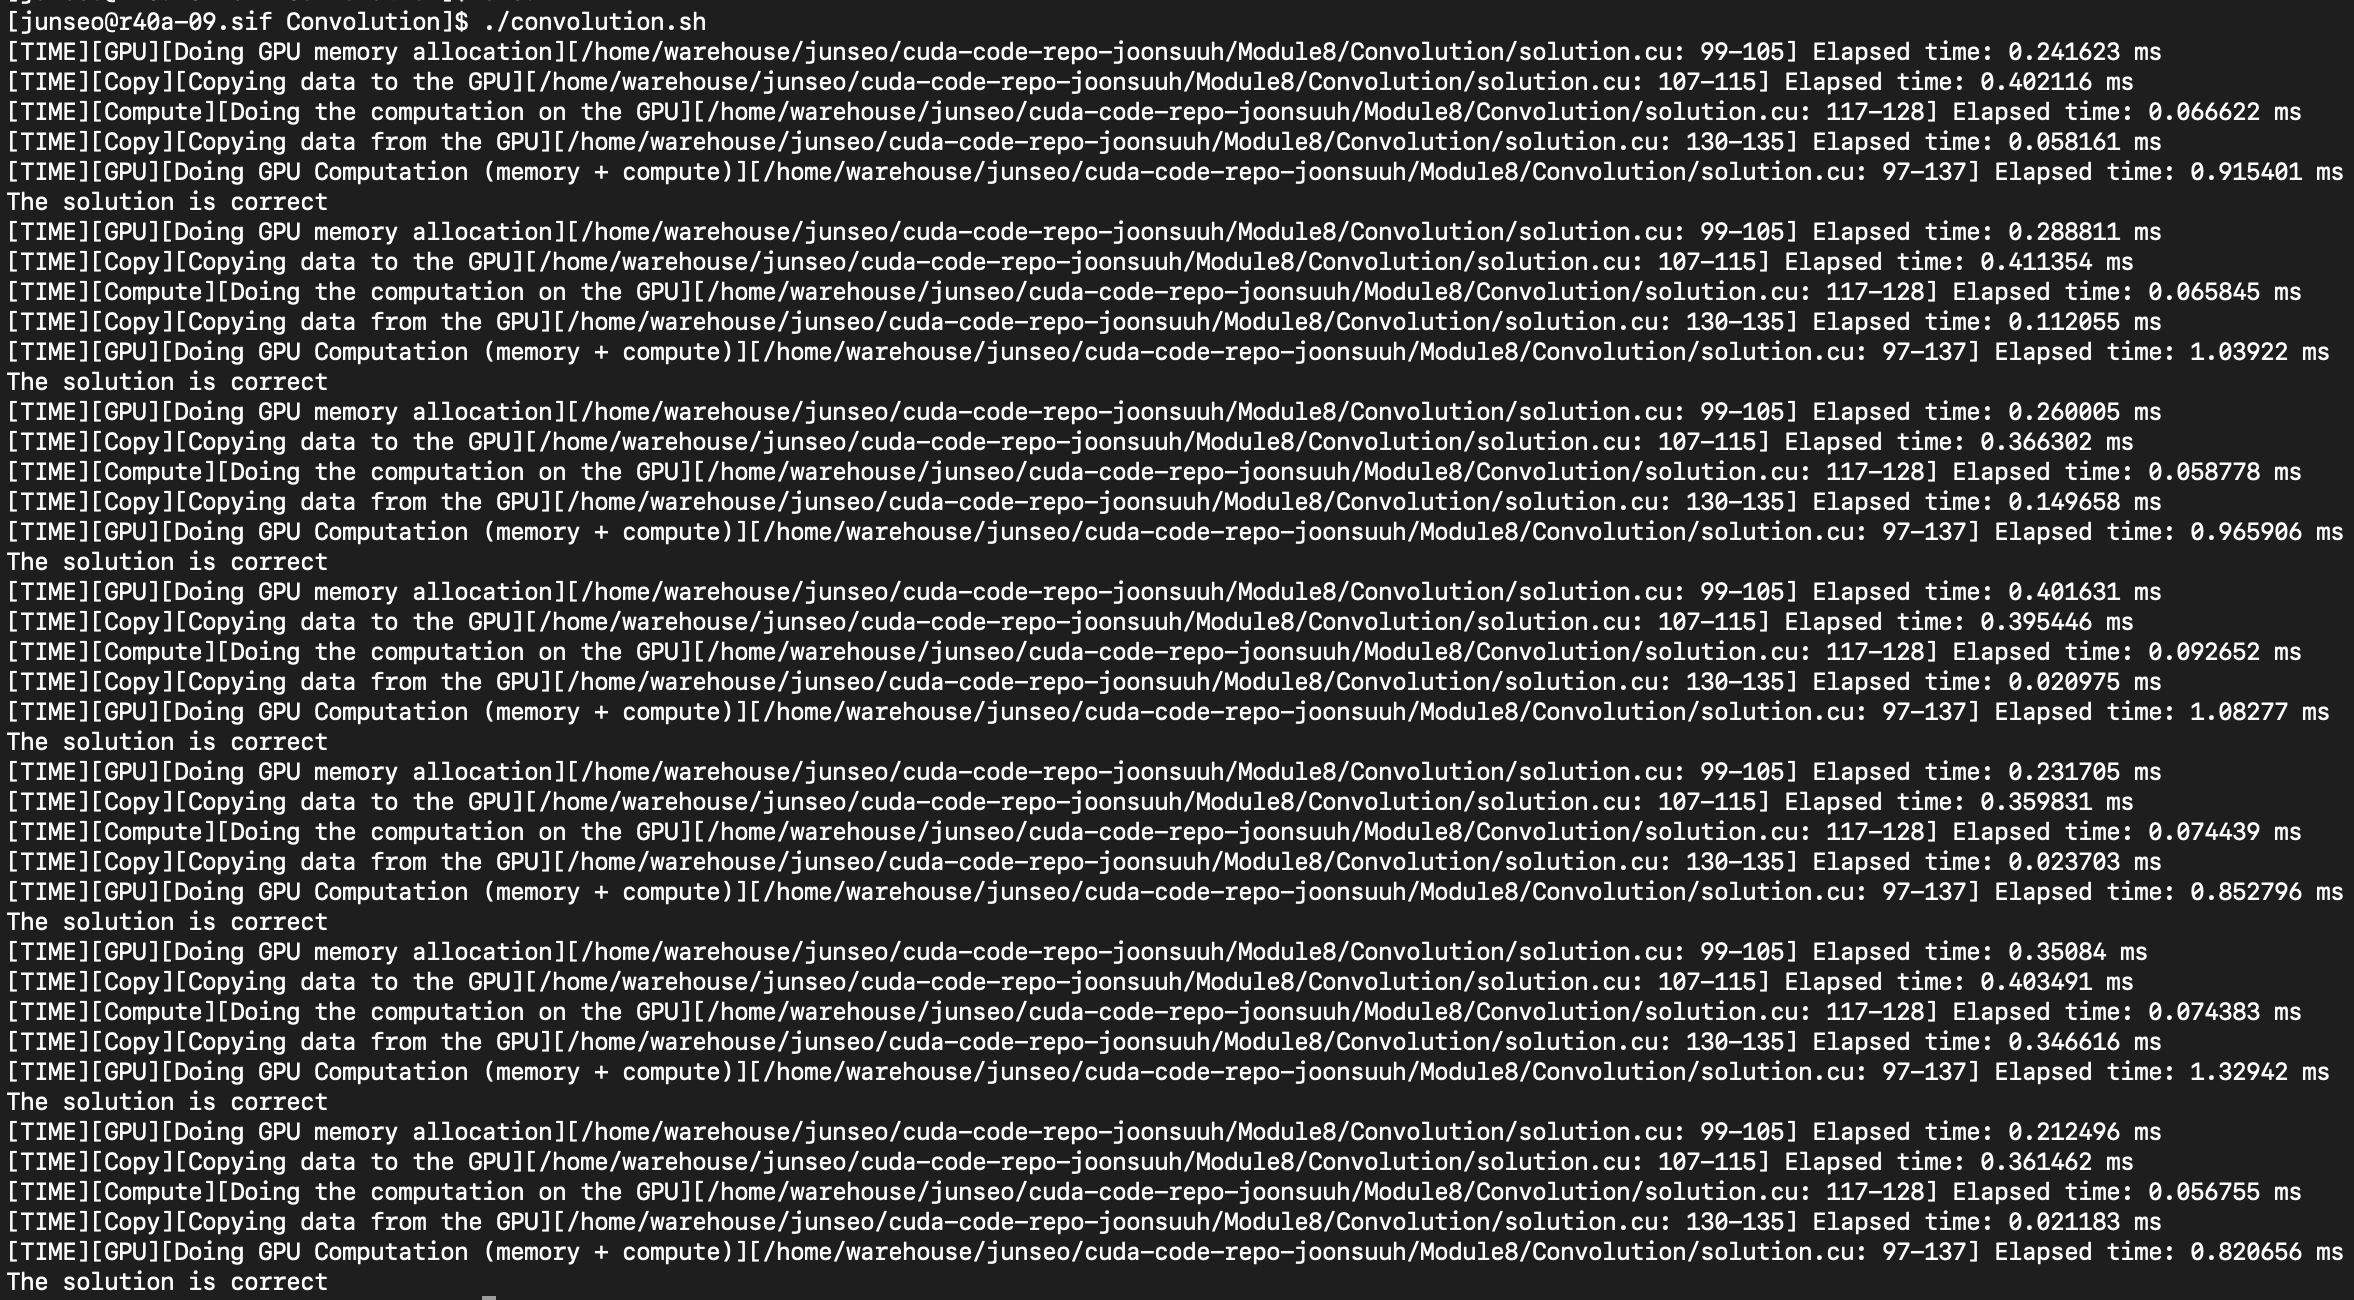
\includegraphics[width=\textwidth]{convolution.png}
    \caption{Convolution}
    \label{fig:convolution}
\end{figure*}
\end{document} 